\documentclass[12pt,openright,twoside,a4paper]{book}
\usepackage{hyperref}
\usepackage[T1]{fontenc}
\usepackage[utf8]{inputenc}
\usepackage[italian]{babel}
\usepackage{amsmath}
\usepackage{amssymb}
\usepackage{caption}
\usepackage{graphicx}
\usepackage{booktabs}
\usepackage{textcomp}


% permette di inserire le note a margine
\usepackage{marginnote}


\begin{document}
\frontmatter
\tableofcontents
\mainmatter

\chapter{Supervised Learning e Metodi Statistici}

\section{Introduzione al Supervised Learning}
La scienza delle predizioni, o data learning, gioca un ruolo chiave in diversi campi scientifici come ad esempio quello della statistica e dell'intelligenza artificiale, grazie a procedure applicative legate principalmente al cosiddetto data mining.

In un tipico scenario di apprendimento supervisionato è presente un valore di \textit{outcome}, generalmente quantitativo (come ad esempio una quotazione finanziaria) o categorico (come ad esempio una discriminante situazionale del tipo infarto/non infarto), che si vuole predire in base ad un set \textit{features} (ad esempio dati clinici).
Avendo a disposizione un \textit{training set} di dati, dei quali è possibile osservare outcome e features per un insieme di oggetti (ad esempio una popolazione), è dunque opportuno costruire un modello predittivo, o \textit{learner}, il quale permetterà di valutare l'outcome per oggetti ignoti.

Una situazione di questo tipo è detta di \textit{Supervised Learning} in quanto è la presenza della variabile di outcome a guidare l'intero processo di apprendimento.
Introducendo un linguaggio più vicino al \textit{machine learning}, è possibile schematizzare il problema nel seguente semplice modo: si ha a che fare con un set di variabili in \textit{input}, generalmente misurate o note a priori, le quali influenzano uno o più \textit{outputs}; l'obiettivo è l'utilizzo degli input per la previsione dei valori in output.

\section{Interpolazioni Lineari e Maximum Likelihood}
Tra i metodi più ampiamente utilizzati per la costruzione di \textit{learners} troviamo quelli che appartengono alla macrocategoria della Maximum Likelihood, ossia che tendono a massimizzare la cosiddetta funzione di verosimiglianza, definita in base alla probabilità di osservare una data realizzazione campionaria dipendentemente ai valori assunti dai parametri statistici oggetto di stima.

La bontà delle predizioni effettuate con questi metodi può essere quantificata in vari modi.
Uno dei più importanti è rappresentato dalla distinzione \textit{Precisione} ed \textit{Accuratezza}.
L'accuratezza rappresenta quanto è distorta la predizione; una predizione è accurata quando il valore atteso dato dalla tecnica non ha \textit{Bias}, ovvero è vicino al valore teorico.
La precisione rappresenta la variabilità (\textit{Variance} in inglese) della predizione; un metodo con alta precisione avrà poca dispersione intorno al proprio valore atteso.
In generale non è possibile ottimizzare entrambe allo stesso momento, ed è quindi necessario scegliere il metodo più appropriato in base alle proprie esigenze.

\begin{figure}[!h]
\centering
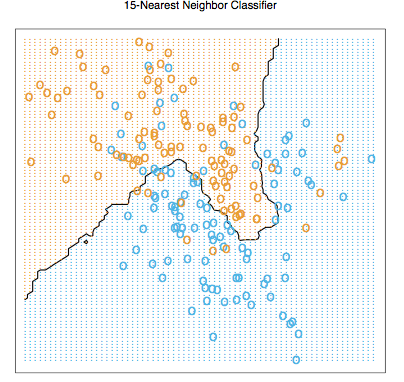
\includegraphics[width=0.45\linewidth]{neighclass}
\caption{\textit{Esempio di problema di classificazione binaria (Blue=0, Orange=1) elaborato tramite K-Nearest Neighbor Prediction}}
\label{neighclass}
\end{figure}

\begin{figure}[!h]
\centering
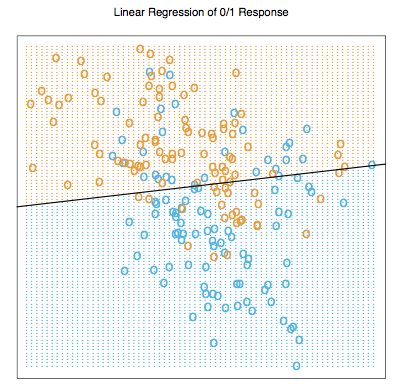
\includegraphics[width=0.45\linewidth]{linclass}
\caption{\textit{Esempio di problema di classificazione binaria (Blue=0, Orange=1) elaborato tramite interpolazione lineare}}
\label{linclass}
\end{figure}

La potenza e la popolarità dei metodi appartenenti alla classe della Maximum Likelihood è dovuta alla relativa semplicità analitica e ad una buona stabilità nella realizzazione delle soluzioni predittive.
Due ottimi esempi di ciò sono i metodi di \textit{K-nearest Neighbor Prediction} e di \textit{Interpolazione Lineare per Minimi Quadrati (Least Squares)}; il primo fornisce soluzioni precise a partire da assunzioni strutturali poco stringenti, dunque in generale meno stabili (\textit{High Variance, Low Bias}) (figura \ref{neighclass}).
Il secondo presuppone assunzioni strutturali più consistenti, il che conduce ad una stabilità maggiore nei risultati a scapito di una minore precisione (\textit{Low Variance, High Bias)}(figura \ref{linclass}).

Per gli scopi del processo utilizzato nella produzione dei risultati relativi a questo lavoro, è opportuna una trattazione analitica più dettagliata di quest'ultimo metodo.

\subsection{Modelli Lineari e Minimi Quadrati}
Il modello lineare è uno dei capisaldi delle analisi statistiche ed anche in ambito di machine learning costituisce un potente strumento d'indagine.
Si giustificherà infatti in questa sezione il fatto che sia possibile ottenere risultati adeguati e facilmente interpretabili anche avendo a disposizione piccoli datasets o in presenza di un basso rapporto segnale-rumore, rendendo dunque il modello lineare altamente performante in termini di capacità predittiva anche in confronto a modelli più analiticamente complessi.

Dato un vettore di inputs  $X^T = (X_1,X_2,...,X_n)$, intendiamo predire l'output $Y$ attraverso il modello
\begin{equation}
\hat{Y}=\hat{\beta_0}+\sum_{j=1}^{n}X_j\hat{\beta_j}
\end{equation}

dove il termine $\hat{\beta_0}$ è l'intercetta o \textit{bias} in termini di machine learning.
$X$ può essere una qualsiasi combinazione delle variabili usate per la predizione, lineare o meno; il termine
modello lineare si riferisce infatti solo ai coefficienti $\beta_j$.

Al fine di creare una notazione più compatta possiamo includere la variabile costante $1$ in $X$ e $\hat{\beta_0}$ in $\hat{\beta}$, vettore dei coefficienti associati. Avremo ora la seguente formulazione per il modello
\begin{equation}
\hat{Y}=X^T\hat{\beta}
\end{equation}
dove $X^T$ denota il vettore o la matrice trasposta (essendo $X$ un vettore colonna).

Nell'occorrenza in cui l'output sia unico $Y$ sarà uno scalare; in generale può però consistere di un vettore \textit{K-dimensionale}, nel qual caso $\beta$ assumerebbe la forma di una matrice di coefficienti a dimensione $n\times K$.

Vedendola come funzione nello spazio \textit{n-dimensionale} degli input $f(X)=X^T\beta$ è lineare ed il gradiente $f'(X)=\beta$ è un vettore dello spazio degli input con direzione e verso concordi con la direzione di massima pendenza.

Per il fitting del modello lineare su un training set di dati, verrà analizzato il metodo detto dei \textit{minimi quadrati}.
Questo approccio ha come obiettivo quello di trovare i coefficienti $\beta$ che minimizzano la \textit{somma quadratica dei residui}, definita da
\begin{equation}
RSS(\beta)=\sum_{j=1}^{N}(y_i-x_i^T\beta)^2
\end{equation}

La funzione $RSS(\beta)$ è una funzione quadratica dei parametri; essa ammette sempre dunque un minimo, ma non è scontata l'unicità di quest'ultimo.
Utilizzando un'agevole notazione matriciale per caratterizzare la soluzione abbiamo
\begin{equation}
RSS(\beta)=(\textbf{y}-\textbf{X}\beta)^T(\textbf{y}-\textbf{X}\beta)
\end{equation}

dove \textbf{X} è una matrice $N \times n$ le cui righe sono vettori di input e \textbf{y} è un vettore \textit{N-dimensionale} di outputs nel training set.

Differenziando per $\beta$ si ottiene l'\textit{equazione normale}
\begin{equation}
\textbf{X}^T(\textbf{y}-\textbf{X}\beta)=0
\end{equation}

nell'ipotesi in cui $\textbf{X}^T\textbf{X}$ sia non singolare, la soluzione unica è data da
\begin{equation}
\hat{\beta}=(\textbf{X}^T\textbf{X})^{-1}\textbf{X}^T\textbf{y}
\end{equation}

il valore interpolato per l'\textit{i}esimo punto di input $x_i$ sarà dunque $\hat{y}(x_i)=x_i^T\hat{\beta}$. Per un arbitrario punto $x_0$ avremo dunque una previsione data da $\hat{y}(x_0)=x_0^T\hat{\beta}$. \cite{ESL}
Qualora $X^TX$ risultasse singolare una delle osservabili contenute in $X$ sarebbe esprimibile come una combinazione lineare di altri osservabili, ovvero $X$ non sarebbe di rango massimo. Anche nel caso in cui questo non fosse esattamente vero, matrici quasi singolari potrebbero comunque dare problemi di convergenza agli algoritmi normalmente utilizzati.

Nel caso ad esempio in cui la funzione interpolante desiderata debba essere una semplice retta $y=bx+a$ (regressione lineare) vanno determinati univocamente i parametri $a$ e $b$ in modo da soddisfare il problema di minimizzazione generale, che si riduce alla minimizzazione della distanza euclidea tra le due successioni,$y_i$ e $f(x_i)$ data da
\begin{equation}
 S = \sum_{i=1}^n \left(y_i - f(x_i)\right)^2
\end{equation}

È possibile in tal caso esplicitare i coefficienti $a$ e $b$ come
\begin{equation}
b=\frac{ N \sum (x_i y_i) - \sum x_i \sum y_i}{N\sum (x_i^2)-(\sum x_i)^2}
\end{equation}

\begin{equation}
a=\frac{\sum y_i \sum (x_i^2)- \sum (x_i) \sum (x_i y_i)}{N\sum (x_i^2)-(\sum x_i)^2}
\end{equation}

Le ipotesi necessarie sono che i residui ($y-f(x)$) seguano una distribuzione normale (o approssimabile come tale); che sia cioè $x_{i}\sim N(\mu,\sigma^{2}), \forall i$, e che la grandezza $Y$ sia a queste ragionevolmente correlata come $Y=A+BX$ . 
Queste garantiscono che il metodo dei minimi quadrati permetta di calcolare esattamente i parametri $\mu$ e $\sigma$ per la distribuzione, essendo questo la \textit{soluzione analitica} al problema della \textit{maximum likelihood} per una Gaussiana.

Con un ragionamento più generale, assumiamo infatti di dover cercare una correlazione qualsiasi del tipo $Y=\Phi(X)$; essa dipenderà da un certo numero di parametri in modo tale che si possa scrivere
\begin{equation}
Y=\Phi(X,\{\lambda_k\})
\end{equation}

Per la stima dei parametri $\{\lambda_k\}$ e quindi per l'adattamento della funzione $Y=\Phi(X,\{\lambda_k\})$ ai punti sperimentali introduciamo due ipotesi di partenza:
\begin{itemize}
\item L'incertezza su $X$ è trascurabile rispetto all'incertezza su $Y$
\item L'incertezza su $Y$ è espressa in termini dello scarto quadratico medio di una distribuzione normale, cioè $\delta y_i=\sigma_i$
\end{itemize}

Se i parametri $\{\lambda_k\}$ della funzione $Y=\Phi(x,\{\lambda_k\})$ fossero noti, una volta fissato un valore $x_i$ della variabile indipendente $X$, la densità di probabilità di misurare un valore $y_i$ sarebbe
\begin{equation}
f(y_i)=\frac{1}{\sigma_i \sqrt{2\pi}} exp\{- \frac{[y_i - \phi(x,\{\lambda_k\})]^2}{2\sigma_i^2}\}
\end{equation}

Fissato un insieme di $N$ valori $x_1,..,x_N$ di $X$, la densità di probabilità di ottenere una $N-pla$ di valori $y_1,...,y_N$ tra loro indipendenti è data da una densità multivariata fattorizzabile nel prodotto delle singole densità $f(y_i)$

\begin{equation}
g(y_1,...,y_N;\{\lambda_k\})=\prod^{N}_{i=1}\frac{1}{\sigma_i \sqrt{2\pi}} exp\{- \frac{[y_i - \phi(x,\{\lambda_k\})]^2}{2\sigma_i^2}\}
\end{equation}

\begin{equation}
g(y_1,...,y_N;\{\lambda_k\})=\frac{1}{(\prod_{i}\sigma_i)(2\pi)^{N/2}} exp\{-1/2\sum^{N}_{i=1} \frac{[y_i - \phi(x,\{\lambda_k\})]^2}{\sigma_i^2}\}
\end{equation}


Nella realtà sono invece noti gli $N$ valori $y_i$, mentre sono incogniti i valori dei parametri $\{\lambda_k\}$.

Le migliori stime dei parametri si hanno ora massimizzando $g(y_1,...,y_N;\{\lambda_k\}$ rispetto ad essi, ossia minimizzando la sommatoria che compare all'esponente dell'ultimo membro dell'equazione di cui sopra.
Questo rappresenta la scelta dei parametri $\lambda_k$ tali che i dati osservati siano il più plausibile possibile.

La sommatoria viene convenzionalmente indicata come $\chi^2$

\begin{equation}
\chi^2=\sum^{N}_{i=1} \frac{[y_i - \phi(x,\{\lambda_k\})]^2}{\sigma_i^2}\}
\end{equation}

Essendo ora noti i valori $x_i$ e $y_i$ e $\sigma_i$ è chiaro che la funzione $\chi^2$ è una funzione dei soli parametri $\{\lambda_k\}$
\begin{equation}
\chi^2=\chi^2(\lambda_1,...,\lambda_p)
\end{equation}

definita in uno spazio \textit{p-dimensionale}.

Per determinare i $\{\lambda_k\}$ che permettono alla funzione $\Phi(x,\{\lambda_k\})$ di adattarsi meglio ai punti sperimentali è sufficiente una minimizzazione di $\chi^2$ nello spazio \textit{p-dimensionale} dei parametri. \cite{fornasini}

E' importante tenere presente che questo tipo di trattazione non prescinde mai dall'ipotesi di normalità

E' necessario tuttavia per lo scopo finale di questo lavoro, analizzare il comportamento della funzione di massima verosimiglianza in presenza di una distribuzione Gaussiana troncata deterministicamente, a partire dalle generalità del metodo.
Nella prossima sezione si giustificherà il fatto che i minimi quadrati non siano più ottimali per la previsione nel caso in cui non siano soddisfatte le condizioni strutturali di normalità.

Ciò accade ad esempio quando si ha a che fare, come nel caso dell'ambito applicativo di questo lavoro, con problemi relativi alla mancanza dei dati \textit{(Missing Data Problems)}.
Vi sono molteplici classificazioni dei problemi relativi ai dati mancanti; alla luce dell'analisi che sarà svolta nel successivo capitolo è necessario approfondire il caso in cui la mancanza dei dati sia deterministica, dunque non randomica (\textit{Missing not at Random}).

In generale l'assenza di dati riduce la rappresentatività del campione, inferendo negativamente sui risultati relativi alla popolazione.
In situazioni dove è previsto questo tipo di problema, è auspicabile utilizzare metodi di analisi \textit{consistenti}, ossia che tengano conto del fatto che piccole violazioni sulle assunzioni strutturali del metodo utilizzato producano un risultato finale comunque poco soggetto a\textit{biases}.

Alcune delle soluzioni più comuni a casistiche di questo tipo riguardano ad esempio tecniche di \textit{sostituzione (imputations)} dei dati mancanti (si vedano i metodi di \textit{partial imputation, partial deletion}), o tecniche di \textit{interpolazione}, cioè di costruzione di nuovi punti sperimentali all'interno del range discreto di dati acquisiti. \cite{Mdata}

Tuttavia, nel caso presente il problema non è affrontabile con metodi canonici in quanto i dati sono esclusi deterministicamente a causa di un criterio di selezione delle popolazioni.

Anche i metodi che discriminano le possibili ragioni della mancanza dei dati, le cosiddette \textit{Model Based Techniques} non sono funzionali alla risoluzione.
Essi infatti richiedono che per la variabile $Y$, contenente la spiegazione della mancanza delle osservazioni in $X$, qualora avesse anch'essa dei valori mancanti, la ragione della mancanza di questi sia casuale. \cite{Mdata}

Il problema della mancanza completa di dati al di fuori di un intervallo, a causa di un criterio di selezione, riguarda pertanto la distorsione dei risultati dipendentemente dal fatto che la mancanza di un dato è strettamente associata al suo stesso valore, ovviamente per ragioni sperimentali.

La soluzione che questo lavoro propone è infatti relativa alla quantificazione dell'effetto di troncamento e all'introduzione di metodi di elaborazione analiticamente giustificati.

\subsection{Maximum Likelihood e Distribuzioni Normali Troncate}
L'ipotesi strutturale sulla distribuzione dei residui, necessaria per l'assunzione dei minimi quadrati come funzione di massima verosimiglianza, viene meno nel caso in cui si ha a che fare con una Gaussiana troncata.

In generale è infatti presente un campionamento $x_1,x_3,..,x_n$ di $n$ osservazioni indipendenti ed identicamente distribuite, provenienti da una distribuzione la cui \textit{funzione di densità di probabilità }  $f_0(\cdot)$ non è nota.
E' comunque assunto che essa appartenga ad una certa famiglia di distribuzioni $ \{f(\cdot |\theta),\theta\in\Theta\} $, dove $\theta$ è un vettore di parametri per la famiglia stessa detta \textit{modello parametrico}, cosicché $f_0=f(\cdot |\theta_0)$.
Il valore $\theta_0$ non è noto ed è il \textit{valore vero} del vettore dei parametri.
E' necessario trovare un estimatore $\hat{\theta}$ il più vicino possibile al valore $\theta_0$.

Per utilizzare il metodo di massima verosimiglianza, si procede specificando la \textit{funzione di densità complessiva} per tutte le osservazioni.
Per un campionamento indipendente e distribuito identicamente si ha
\begin{equation}
f(x_1,x_2,\ldots,x_n\mid\theta) = f(x_1|\theta)\times f(x_2|\theta) \times \cdots \times  f(x_n|\theta)
\end{equation}

Considerando le osservazioni $x_1,x_3,..,x_n$ come parametri fissati della funzione, $\theta$ assumerà il ruolo di variabile arbitraria; è così possibile introdurre la \textit{funzione di verosimiglianza}
\begin{equation}
\mathcal{L}(\theta\,;\,x_1,\ldots,x_n) = f(x_1,x_2,\ldots,x_n\mid\theta) = \prod_{i=1}^n f(x_i\mid\theta)
\end{equation}

Da un punto di vista puramente operativo è conveniente utilizzare il logaritmo della funzione di verosimiglianza (\textit{log-likelihood})
 \begin{equation}
 \ln\mathcal{L}(\theta\,;\,x_1,\ldots,x_n) = \sum_{i=1}^n \ln f(x_i\mid\theta)
 \end{equation}

e considerare il \textit{log-likelihood medio}
\begin{equation}
\hat\ell = \frac1n \ln\mathcal{L}
\end{equation}

La notazione $\hat\ell$ non è affatto casuale: essa assimila il termine ad un estimatore, cosa che in effetti $\hat\ell$ è in quanto indice di verosimiglianza logaritmica attesa per la singola osservazione.

Il metodo di massima verosimiglianza stima dunque $\theta_0$ a partire da un valore $\theta$ che massimizza $\hat\ell(\theta,x)$.

Il metodo definisce così un \textit{Maximum-Likelihood Estimator (\textbf{MLE}) } per $\theta_0$
\begin{equation}
\{ \hat\theta_\mathrm{mle}\} \subseteq \{ \underset{\theta\in\Theta}{\operatorname{arg\,max}}\ \hat\ell(\theta\,;\,x_1,\ldots,x_n) \}
\end{equation}

La massimizzazione della log-likelihood è equivalente a quella della likelihood vera e propria, essendo il logaritmo una funziona monotona strettamente crescente. \cite{MLE}

Per la maggior parte dei modelli, può essere trovato un MLE sotto forma di funzione esplicita dei dati osservati $x_1,x_3,..,x_n$.
Qualora non fosse possibile una trattazione analitica della soluzione di massimizzazione, si utilizzano metodi numerici di ottimizzazione per il MLE.

Il problema dello slicing deterministico dei dati che questo lavoro si propone di affrontare, rende inevitabile la trattazione della distribuzione Gaussiana troncata.

A partire dalla formulazione della sua particolare \textit{funzione di densità di probabilità} sarà possibile giustificare l'impossibilità di definire una soluzione analitica per questo tipo di distribuzioni.

Supponiamo infatti che  $X \sim N(\mu, \sigma^{2}) \!$ abbia una distribuzione normale e sia confinata nell'intervallo $ X \in (a,b), \; -\infty \leq a < b \leq \infty $.
L'aggiunta di queste  condizioni rende la distribuzione $X$ una \textit{Gaussiana troncata} nell'intervallo
$a<X<b$.

La sua funzione di densità di probabilità $f$ per $a\leq x \leq b$ assumerà dunque la forma
\begin{equation}
f(x;\mu,\sigma,a,b) = \frac{\phi(\frac{x - \mu}{\sigma})}{\Phi(\frac{b - \mu}{\sigma}) - \Phi(\frac{a - \mu}{\sigma}) }{.}\frac{1}{\sigma}
\end{equation}

ed $f=0$ al di fuori dell'intervallo.

Si ha che per $	\xi=\frac{x-\mu}{\sigma}$; ${\phi(\xi)=\frac{1}{\sqrt{2 \pi}}\exp{(-\frac{1}{2}\xi^2})} $ rappresenta la funzione di densità di probabilità della \textit{distribuzione normale standard} mentre le ${\Phi(\cdot)}$ sono le \textit{funzioni di distribuzione complessiva (cumulative distribution functions)}. \cite{TGMLE}

La presenza delle $\Phi(\alpha),\Phi(\beta)$ con $\alpha=\frac{a-\mu}{\sigma}, \beta=\frac{b-\mu} {\sigma}$ comporta l'impossibilità di una formulazione semplice ed analiticamente definita dei parametri di massima verosimiglianza, rendendo necessaria un'ottimizzazione numerica per l'approssimazione delle soluzioni.
Questo aspetto e la proposta di possibili metodi di soluzione sono ampiamente trattati in letteratura. \cite{econ}

Questo lavoro si propone tuttavia di correggere i metodi lineari canonici, ampiamente utilizzati dagli algoritmi di \textit{machine learning}, trattando la possibilità di stimare il \textit{bias} associato all'utilizzo di un MLE non analiticamente corretto.

In questo modo sarà possibile ottenere previsioni e risultati verosimili mantenendo la semplicità operativa propria dell'ipotesi lineare.
A questo proposito nella sezione successiva seguirà la descrizione dei metodi legati al machine learning propriamente detto.

\subsection{Train-Test Split e Cross Validation}
Tra le procedure più elementari per un approccio di machine learning alla trattazione dei dati, vi è quello del cosiddetto \textit{train and test splitting}.

Esso consiste nella divisione casuale del dataset in due subsets: \textit{train set} e \textit{test set}.
Il train set, come il nome suggerisce, è utilizzato per elaborare i parametri utilizzando il regressore scelto.
Questi vengono poi applicati e confrontati coi dati presenti nel train set, i quali ovviamente fungendo da dati "non visti" forniscono una stima realistica della performance predittiva del regressore utilizzato, generalmente sotto forma di $R^2$

Operativamente è possibile effettuare lo splitting utilizzando algoritmi di random sorting, fornendo le percentuali di dati da utilizzare come train e test; convenzionalmente si pone la percentuale del train al $70-80\%$ dell'intero dataset, a cui segue quella del test per sottrazione.

Questa procedura, seppur elementare, sopperisce al problema del cosiddetto \textit{overfitting}, ossia la tendenza a creare un modello analitico che interpoli molto precisamente i dati sperimentali a scapito di una scarsa capacità predittiva.

Un metodo direttamente basato sul train-test splitting è quello della \textit{Cross Validation}.
Questo è probabilmente il metodo più semplice ed ampiamente utilizzato per stimare l'errore e dunque la qualità di una predizione.

La cross-validation stima in maniera diretta l'errore atteso per l'analisi riferita al subsample (che possiamo assimilare ad un test set) che rimane esterno all'elaborazione dei parametri, definito come
\begin{equation}
Err=E[L(Y,\hat{f}(X)]
\end{equation}

dunque \textit{l'errore medio generalizzato} relativo all'applicazione del metodo $\hat{f}(X)$ su un test set indipendente appartenente alla distribuzione correlata di $X$ e $Y$.

Idealmente, avendo a disposizione un numero sufficientemente grande di dati, potremmo isolare quello che verrà chiamato \textit{validation set} ed utilizzarlo per valutare la performance del modello predittivo utilizzato.

Tuttavia in generale si hanno a disposizione database non molto estesi, per cui questa procedura risulterebbe approssimativa.

Per sopperire al problema, si introduce la cosiddetta \textit{K-fold cross validation}, la quale usa una parte dei dati per essere interpolati dal modello scelto e un'altra per testarne le capacità predittive.

Si introduce uno splitting dei dati in $K$ parti uguali; per ogni $k-esima$ parte, utilizziamo le rimanenti $k-1$ parti per il fitting del modello e sfruttiamo questa per la stima dell'errore sulla predizione.
Per una descrizione quantitativa si introducono le funzioni seguenti.

Sia $k:\{1,2,...,N\}\longmapsto\{1,...,K\}$ una funzione di indexing che indica la partizione alla quale l'\textit{i-esima} osservazione è assegnata casualmente.

Sia $\hat{f}^{-k}(x)$ la funzione interpolata, calcolata avendo rimosso la \textit{k-esima} parte dei dati.
Allora la stima dell'errore sulla predizione data dalla cross validation sarà
\begin{equation}
CV(\hat{f})=\frac{1}{N}\sum^{N}_{i=1}L(y_i,\hat{f}^{-k(i)}(x_i))
\end{equation}

Delle scelte tipiche per $K$ sono $K=5,K=10$; il caso in cui si ponga $K=N$ la procedura prende il nome di \textit{leave-one-out cross-validation} e si avrà che $k(i)=i$, cosicché per ogni \textit{i-esima} osservazione il fit sarà calcolato su tutte le altre osservazioni eccetto la \textit{i-esima}.

Dato un set di modelli $f(x,\alpha)$ indicizzati tramite il parametro di curvatura $\alpha$, si indica con $\hat{f}^{-k}(x,\alpha)$ l'$\alpha-esimo$ elaborato avendo rimosso la \textit{k-esima} parte dei dati.
Per questo set di modelli definiamo allora

\begin{equation}
CV(\hat{f}(x,\alpha))=\frac{1}{N}\sum^{N}_{i=1}L(y_i,\hat{f}^{-k(i)}(x_i,\alpha))
\end{equation}

La funzione $CV(\hat{f}(x,\alpha))$ fornisce una stima della curva di errore sul test; possiamo così trovare il parametro di \textit{tuning} $\hat{\alpha}$ che la minimizza. Il modello finale scelto per il fit completo dei dati sarà così $f(x,\hat{\alpha})$. \cite{ESL}

\begin{figure}[!h]
\centering
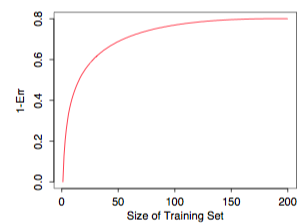
\includegraphics[width=0.5\linewidth]{LearningCurve}
\caption{\textit{Curva di learning ipotetica per un classificatore su una data analisi: si hanno il plot di $1-Err$ contro la dimensione $N$ del training set. Come si può notare vi sono dimensioni dei subsets per cui la cross-validation sovrastima l'errore sulla predizione, a causa della forte pendenza della curva. }}
\label{curve}
\end{figure}

E' interessante a questo punto commentare le capacità performative della cross validation al variare della scelta di $K$.

Per $K=N$ si otterranno stime per l'errore di predizione atteso con un bias praticamente nullo, ma a causa della probabile similitudine reciproca degli $N$ training sets potrebbero presentare un'alta varianza.

Al contrario per $K=5$ ad esempio la varianza sarà bassa, ma il bias potrebbe costituire un problema a causa della sua dipendenza dalla performance del metodo di learning che varia con le dimensioni di train e test sets.

In sintesi, se la curva di learning ha un pendenza considerevole ad una certa dimensione di train o test set, la \textit{k-fold cross-validation} con $K=10,5$ sovrastimerà l'errore sulla predizione.

Il metodo \textit{leave-one-out} ha invece in generale un basso bias ma non è esclusa la possibiità di avere una varianza considerevole.

\chapter{Valutazione degli effetti di troncatura}

\section{Introduzione al Problema}
L'utilizzo di database spesso composti su un intervallo discreto di una data popolazione, frequentemente selezionato tramite criteri che possiamo definire "deterministici" (un intervallo di età ad esempio, o in generale un certo range di valori disponibile al momento dell'acquisizione), si contrappone all'esigenza di ottenere un modello di validità generale in termini di coefficienti delle variabili e di interazione fra esse.

Nella sezione precedente è stato dimostrato come la presenza di una troncatura renda l'utilizzo del metodo dei minimi quadrati (comunque ampiamente utilizzato per elaborazioni di questo tipo) analiticamente non valido.
Una conseguenza inevitabile di ciò è una propagazione dell'errore anche nell'ambito di attribuzione dello score dei modelli ipotetici, poiché avremo una valutazione della bontà di previsione sotto forma di $R^2$ riferita ad un metodo il cui limite di validità è trasceso.

Non è pertanto possibile elaborare un risultato che abbia la pretesa di essere generale senza tenere conto di un'analisi quantitativa dell'effetto di slicing dei set di dati, che come è dimostrato in seguito potrà fornire una correzione applicabile al modello come stima di un bias per i coefficienti in relazione alla percentuale di dati utilizzati nell'elaborazione.

I risultati di seguito riportati si riferiscono ad interpolazioni di tipo lineare, elaborate attraverso metodi di machine learning quali cross-validation e boot-strapping (precedentemente descritti).

\section{Metodi di Elaborazione}

\subsection{Effetto della troncatura nello spostamento della retta di regressione}

Uno degli effetti primari del troncamento dei dati riguarda lo spostamento della retta di regressione rispetto al best fit effettuato nel caso in cui fossero a disposizione i dati nella loro interezza.
Possiamo pensare a questo effetto come se fosse dovuto ad una sorta di \textit{leverage}, ossia ad un fenomeno analogo a quello di una leva che poggia su un fulcro. 

Il metodo dei minimi quadrati ordinario tende infatti a far passare la retta di regressione per il centro dei dati definito come $(\bar{X},\bar{Y})$.
Poichè dunque il metodo mira alla minimizzazione della distanza verticale tra dati e miglior retta di regressione, i punti agli estremi dell'intervallo di $X$ "spingeranno" o "tireranno" più intensamente sulla leva, che in questo caso è la retta data dal best fit.
Si può avere quindi che il peso dei dati nell'elaborazione dei risultati non sia omogeneo.

In termini più legati alla statistica, il risultato di ciò è che la \textit{deviazione standard dei residui}  differisca per differenti punti sperimentali di $X$ anche se la deviazione standard dello stimatore è costante.

\begin{figure}[!h]
\centering
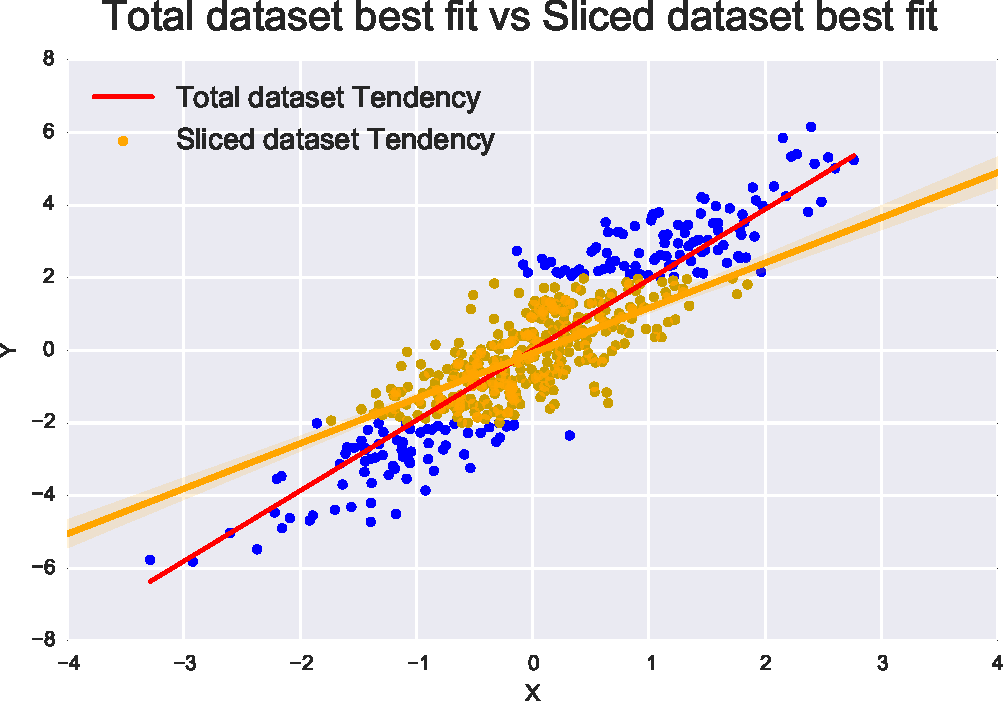
\includegraphics[width=0.6\linewidth]{leverage}
\caption{\textit{In figura è rappresentato il best fit per l'intera popolazione, dato dalla retta in rosso, successivamente troncata in modo da interpolare i soli valori presenti nell'intervallo $-2<y<2$, rappresentato dalla zona arancione nello scatterplot.
Come è evidente, la pendenza della retta di regressione varia notevolmente in relazione all'intervallo di interpolazione.}}
\label{leverage}
\end{figure}

Un'esemplificazione di questo fenomeno è data dalla figura \ref{leverage}, ottenuta dall'interpolazione di due popolazioni $X$ e $Y$, la prima generata casualmente con rumore distribuito normalmente e successivamente troncata in un intervallo definito, la seconda generata come $y=2x$ anch'essa con relativo rumore statistico.

Alla luce di questo effetto così consistente, è necessario approfondire l'analisi dell'effetto di troncatura a livello di \textit{modelling}, quantificandone l'inferenza su elaborazioni relative allo \textit{scoring} e al calcolo dei coefficienti per i parametri di regressione.

\subsection{Generazione delle popolazioni e Data Structures}

Per studiare gli effetti della troncatura della variabile dipendente è stato utilizzato un dataset modello (\textit{toy model}) le cui relazioni sono note e determinate a priori, in modo da poter valutare esattamente gli effetti dei metodi utilizzati nella stima del miglior modello di regressione e del valore dei suoi parametri.

Le popolazioni sintetiche $x_1$,$x_2$,$x_3$ sono generate in modo da essere distribuite normalmente e la $y$ composta secondo la relazione

\begin{equation}
y=x_1+0.1x_1^2+x_2x_3
\label{population}
\end{equation}

con l'aggiunta del relativo rumore statistico, anch'esso simulato normalmente.
In questo modo è possibile valutare la propagazione dell'effetto non solo per termini di primo grado ma anche per  termini di grado superiore al primo e per termini d'interazione (nel caso presente sotto forma di prodotto).

Lo script genera due popolazioni ciascuna composta da $N=10^3$ individui, che successivamente vengono scalate in base alla percentuale di taglio in analisi fornita come argomento alla funzione. Viene fissata una certa percentuale di dati da troncare agli estremi di una popolazione, e l'altra viene generata con un sottocampionamento che mantenga la stessa numerosità ma che rispetti le ipotesi di normalità delle distribuzioni.

In questo modo sarà sempre possibile confrontare risultati elaborati su popolazioni della stessa grandezza, una composta da elementi selezionati casualmente e che dunque sarà semplicemente una "riduzione in scala" della popolazione iniziale, l'altra composta dagli elementi presenti entro il range percentuale del taglio.

Per quest'ultima categoria di campioni lo slicing viene infatti effettuato dallo script non in maniera stocastica, ma previo sorting del dataset secondo percentili relativi alle posizioni delle singole osservazioni nell'array, vengono eliminati dati a partire dalle estremità in base alla percentuale di slicing fornita come argomento in generazione.

Questa procedura permette di imputare le discrepanze attese relativamente al ranking di modelli ipotetici e stima dei parametri per i coefficienti unicamente al bias dovuto al troncamento deterministico del dataset.

Prima di procedere con la descrizione dei metodi analitici, è utile commentare le strutture utilizzate per manipolare i dati in input; cercando di rendere il programma il più generale possibile è stata infatti introdotta un'organizzazione di tipo Design Matrix, oggetti che descrivono la  composizione matriciale per regressioni multivariate.

Sia un modello di regressione nella forma $y=X\beta+\epsilon$ dove $X$ è la design matrix, $y$ il vettore delle osservazioni sulla variabile dipendente, $\beta$ un vettore di coefficienti associati alle $X_i$ ed $\epsilon $ il vettore dei termini di errore.
Prendendo ad esempio un modello del tipo:
\begin{equation}
y_i = \beta_0 + \beta_1 w_i + \beta_2 x_i + \epsilon_i
\end{equation}

con 7 osservazioni dipendenti dalle variabili $w$ ed $x$, si ha in termini matriciali:
\begin{equation}
\begin{bmatrix}y_1 \\ y_2 \\ y_3 \\ y_4 \\ y_5 \\ y_6 \\ y_7 \end{bmatrix} =
\begin{bmatrix} 1 & w_1 & x_1  \\1 & w_2 & x_2  \\1 & w_3 & x_3  \\1 & w_4 & x_4  \\1 & w_5 & x_5  \\1 & w_6 & x_6 \\ 1& w_7  & x_7  \end{bmatrix}
\begin{bmatrix} \beta_0 \\ \beta_1 \\ \beta_2  \end{bmatrix}
+
\begin{bmatrix} \epsilon_1 \\ \epsilon_2 \\ \epsilon_3 \\ \epsilon_4 \\ \epsilon_5 \\ \epsilon_6 \\ \epsilon_7 \end{bmatrix}
\end{equation}

Convenzionalmente, ed anche all'interno del programma utilizzato, la matrice delle $y$ è definita come "Outcome" e quella delle $X$ come "Predictor"; in questo modo è possibile generalizzare l'elaborazione senza dover definire funzioni specifiche in relazione al numero ed al tipo di variabili introdotte.

L'analisi è dunque strutturata in due parti specifiche per valutare l'effetto di slicing su quelli che sono aspetti essenziali per l'attribuzione della capacità predittiva di un dato metodo: il ranking di modelli ipotetici per $y$, ovviamente noto quello utilizzato per la generazione, e la precisione nella stima dei coefficienti per  le $x$.

\subsection{Effetto della troncatura nell'attribuzione dello score per modelli ipotetici}
L'algoritmo utilizzato per questo tipo di analisi prevede l'uso di tecniche di Cross Validation (nel caso specifico K-Fold Cross Validation con un numero di folds pari a 10) per il calcolo della bontà di previsione del regressore fornito.
 
In questo caso è stata introdotta una semplice interpolazione lineare multivariata, con il quale lo script procede ad elaborare un array contenente dei modelli ipotetici, incluso quello utilizzato per la generazione delle $y$ e che può dunque essere preso come riferimento, valutandone un $R^2$ "generalizzato".
Ciò è operativamente realizzabile tramite una popolazione di validazione selezionata casualmente a cui vengono applicati i vari coefficienti calcolati su stratificazioni di popolazioni di Train e Test diverse per ogni iterazione, anch'esse ottenute tramite random shuffling.

In questo modo è possibile simulare l'effetto di perdita di dati sensibili a causa di criteri di selezione dei campioni o in generale l'utilizzo di un range discreto di occorrenze.

L'array dei modelli di prova contiene ipotesi riferite ai singoli termini, a tutte le loro possibili combinazioni lineari, alle possibili interazioni a coppie ed a strutture più vicine al modello di generazione e dunque contenenti termini di grado superiore al primo.
Di seguito sono riportate alcune tabelle di ranking riferite a diverse percentuali di troncatura.

\begin{table}[!h]
\begin{tabular}{lrrrr}
\toprule
{} &  entire &  sliced &  entire val. &  sliced val. \\
\midrule
y$\sim$x2*x3+I(x1**2)+x1 &         0.685 &         0.684 &             0.665 &             0.664 \\
y$\sim$x2*x3+x1          &         0.678 &         0.678 &             0.665 &             0.664 \\
y$\sim$x2*x3             &         0.353 &         0.347 &             0.319 &             0.319 \\
y$\sim$x2*x3+I(x1**2)    &         0.345 &         0.345 &             0.331 &             0.332 \\
y$\sim$x1 + x2           &         0.315 &         0.314 &             0.314 &             0.318 \\
y $\sim$ x1              &         0.311 &         0.312 &             0.323 &             0.322 \\
y $\sim$ x1 * x2         &         0.312 &         0.312 &             0.319 &             0.323 \\
y$\sim$x1+x2+x3          &         0.313 &         0.312 &             0.323 &             0.328 \\
y$\sim$x1+x3             &         0.310 &         0.310 &             0.314 &             0.311 \\
y$\sim$x1*x3             &         0.307 &         0.307 &             0.327 &             0.325 \\
y$\sim$x3                &        -0.009 &        -0.011 &            -0.001 &            -0.002 \\
y $\sim$ x2              &        -0.005 &        -0.011 &            -0.005 &            -0.002 \\
\bottomrule
\end{tabular}
\caption{\textit{La tabella contiene gli scores relativi alle prove per popolazioni intere e tagliate ed i corrispondenti punteggi  ottenuti su popolazioni di validazione, in questo caso senza troncature, per verificare che l'algoritmo restituisse valori consistenti.}}
\end{table}

\begin{table}[!h]
\begin{tabular}{lrrrr}
\toprule
{} &  entire &  sliced &  entire val. &  sliced val. \\
\midrule
y$\sim$x2*x3+I(x1**2)+x1 &         0.659 &         0.260 &             0.665 &             0.494 \\
y$\sim$x2*x3+x1          &         0.646 &         0.256 &             0.664 &             0.482 \\
y $\sim$ x1              &         0.308 &         0.134 &             0.326 &             0.209 \\
y$\sim$x1 + x2           &         0.309 &         0.131 &             0.339 &             0.213 \\
y$\sim$x1+x3             &         0.306 &         0.130 &             0.329 &             0.209 \\
y$\sim$x1*x3             &         0.299 &         0.130 &             0.335 &             0.211 \\
y $\sim$ x1 * x2         &         0.303 &         0.128 &             0.330 &             0.211 \\
y$\sim$x1+x2+x3          &         0.306 &         0.128 &             0.323 &             0.210 \\
y$\sim$x2*x3             &         0.354 &         0.048 &             0.306 &             0.186 \\
y$\sim$x2*x3+I(x1**2)    &         0.352 &         0.042 &             0.338 &             0.192 \\
y $\sim$ x2              &        -0.019 &        -0.013 &            -0.005 &            -0.003 \\
y$\sim$x3                &        -0.023 &        -0.015 &            -0.001 &            -0.001 \\
\bottomrule
\end{tabular}
\caption{\textit{La tabella contiene gli scores relativi alle prove per popolazioni intere e tagliate ed i corrispondenti punteggi  ottenuti su popolazioni di validazione, in questo caso la percentuale di utilizzo del database è del 66\%.}}
\end{table}

\begin{table}[!h]
\begin{tabular}{lrrrr}
\toprule
{} &  entire &  sliced &  entire val. &  sliced val. \\
\midrule
y$\sim$x2*x3+x1          &         0.495 &         0.011 &             0.658 &             0.148 \\
y$\sim$x2*x3+I(x1**2)+x1 &         0.510 &         0.005 &             0.660 &             0.146 \\
y$\sim$x1+x3             &         0.215 &        -0.031 &             0.285 &             0.049 \\
y $\sim$ x1              &         0.218 &        -0.041 &             0.319 &             0.050 \\
y$\sim$x1*x3             &         0.215 &        -0.045 &             0.330 &             0.049 \\
y$\sim$x1+x2+x3          &         0.227 &        -0.047 &             0.269 &             0.046 \\
y$\sim$x2*x3             &         0.117 &        -0.058 &             0.319 &             0.047 \\
y$\sim$x3                &        -0.131 &        -0.058 &            -0.009 &            -0.001 \\
y$\sim$x1 + x2           &         0.231 &        -0.059 &             0.310 &             0.049 \\
y $\sim$ x1 * x2         &         0.225 &        -0.070 &             0.269 &             0.046 \\
y$\sim$x2*x3+I(x1**2)    &         0.094 &        -0.076 &             0.346 &             0.047 \\
y $\sim$ x2              &        -0.094 &        -0.091 &            -0.038 &            -0.005 \\
\bottomrule
\end{tabular}
\caption{\textit{La tabella contiene gli scores relativi alle prove per popolazioni intere e tagliate ed i corrispondenti punteggi  ottenuti su popolazioni di validazione, in questo caso la percentuale di utilizzo del database è del 33\%}.}
\end{table}

\pagebreak

Si può notare come tendenza generale che la valutazione della performance predittiva fornita dalla cross-validation in riferimento all'elaborazione sulle popolazioni troncate (indicate come \textit{sliced} sulle tabelle) sia sempre piuttosto ottimistica; questo fenomeno però non deve trarre in inganno poiché se andassimo ad analizzare l'errore sulla previsione sarebbe anch'esso sovrastimato.
Tutto ciò a causa dell'utilizzo della \textit{ten-fold cross-validation} e dell'andamento generale della \textit{ curva di learning} che come descritto nel paragrafo precedente dipende fortemente dalle dimensioni dei datasets considerati \ref{curve}

Come si vede dai risultati, la classifica dei modelli in relazione alla stima del peso dei termini è in generale mantenuta anche per perdite considerevoli di dati mentre la qualità della previsione riferita alle popolazioni tagliate peggiora notevolmente; resta quindi da determinare l'andamento della stima dei coefficienti in relazione alla percentuale di utilizzo dei datasets.


\subsection{Effetto della troncatura nella stima dei coefficienti }

Per la stima del bias sui coefficienti è stata effettuata come prima analisi uno scatter plot dei pesi dei parametri della popolazione generata considerata interamente, contro quelli ottenuti dopo aver tagliato la suddetta popolazione.

Va tenuto presente che le funzioni utilizzate per questa sezione dell'elaborazione sono le stesse descritte nelle sezioni  2.2.2 per quanto riguarda generazione della popolazione e nella 2.2.3 relativamente allo script di simulazione della troncatura; avremo dunque che i pesi reali associati alle variabili sono dati dalla relazione \ref{population}.

\begin{figure}[!h]
\centering
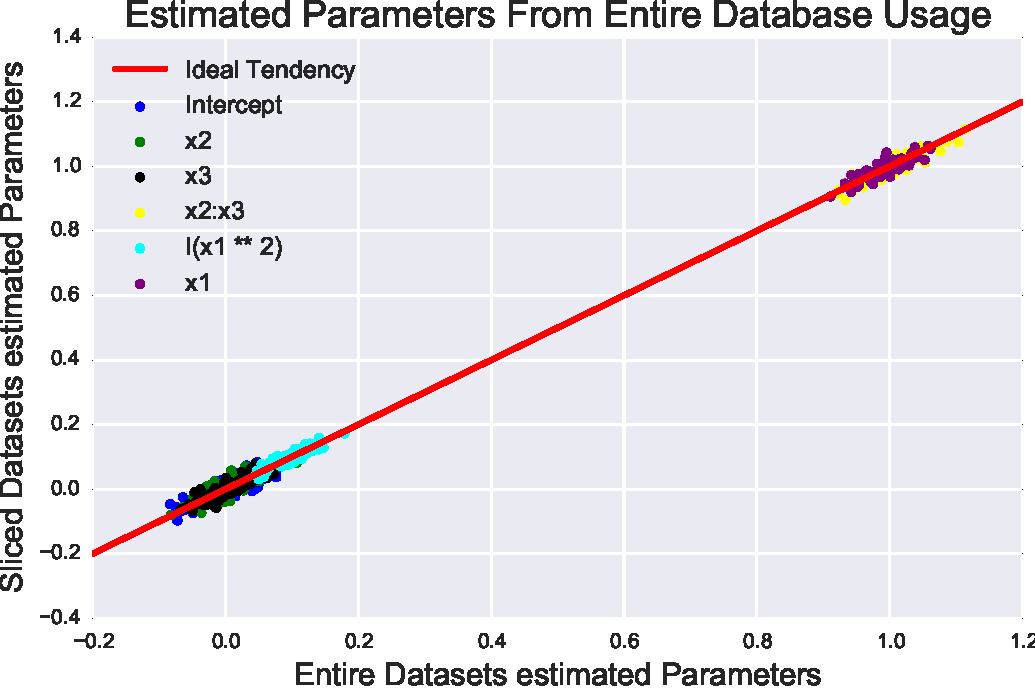
\includegraphics[width=0.55\linewidth]{coeffscatter100}
\caption{\textit{In figura sono rappresentate le dispersioni attorno ai valori riferiti al peso dei coefficienti della popolazione generata. 
In questo caso, non avendo effettuato nessun tipo di taglio, notiamo come nei limiti del rumore statistico simulato i risultati dell'elaborazione siano piuttosto precisi e seguano la tendenza ideale, rappresentata dalla retta in rosso.}}
\label{coeffscatter100}
\end{figure}

 Sono riportate due elaborazioni esemplificative, la prima riferita ad un calcolo basato sull'intero database (figura \ref{coeffscatter100}), la seconda avendo asportato il 30\% della popolazione (figura \ref{coeffscatter70}).

\begin{figure}[!h]
\centering
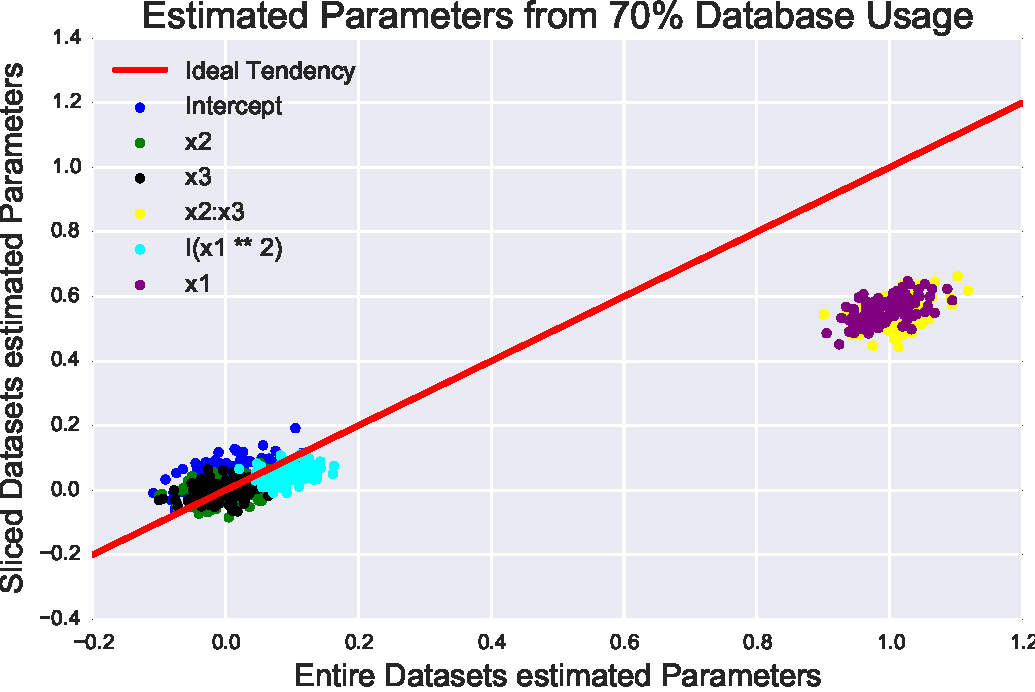
\includegraphics[width=0.55\linewidth]{coeffscatter70}
\caption{\textit{In figura sono rappresentate le dispersioni attorno ai valori riferiti al peso dei coefficienti della popolazione generata. 
In questo caso è stato effettuato un taglio del 30\%; come si nota la dispersione dei pesi per i parametri $x1$ e $x2x3$, ai quali per generazione è associato un peso pari a $1.0$, è già in queste condizioni fortemente deviata rispetto al valore vero e di conseguenza alla tendenza ideale.}}
\label{coeffscatter70}
\end{figure}

Questo primo tipo di analisi, il cui risultato è una visualizzazione qualitativa dell'effetto di slicing, oltre ad essere rappresentativa del fenomeno descritto nella sezione 2.2.1, ha come conseguenza la necessità di quantificare l'andamento della deviazione nella stima dei parametri proporzionalmente alla percentuale di troncatura.

Il processo utilizzato per  questo tipo di indagine è associato al calcolo della variazione del \textit{rapporto tra coefficiente reale e coefficiente stimato}, in relazioni a diverse percentuali di utilizzo del database.

Operativamente sono stati utilizzati tutti gli scripts descritti precedentemente, con l'aggiunta di un metodo che permette di accedere ai parametri per i singoli termini del modello e di un ciclo di elaborazione statstica che consente  di utilizzare mediane e deviazioni standard per il plotting.
I grafici seguenti mostrano l'andamento dei rapporti per steps di slicing del 10\%.

\begin{figure}[!h]
\centering
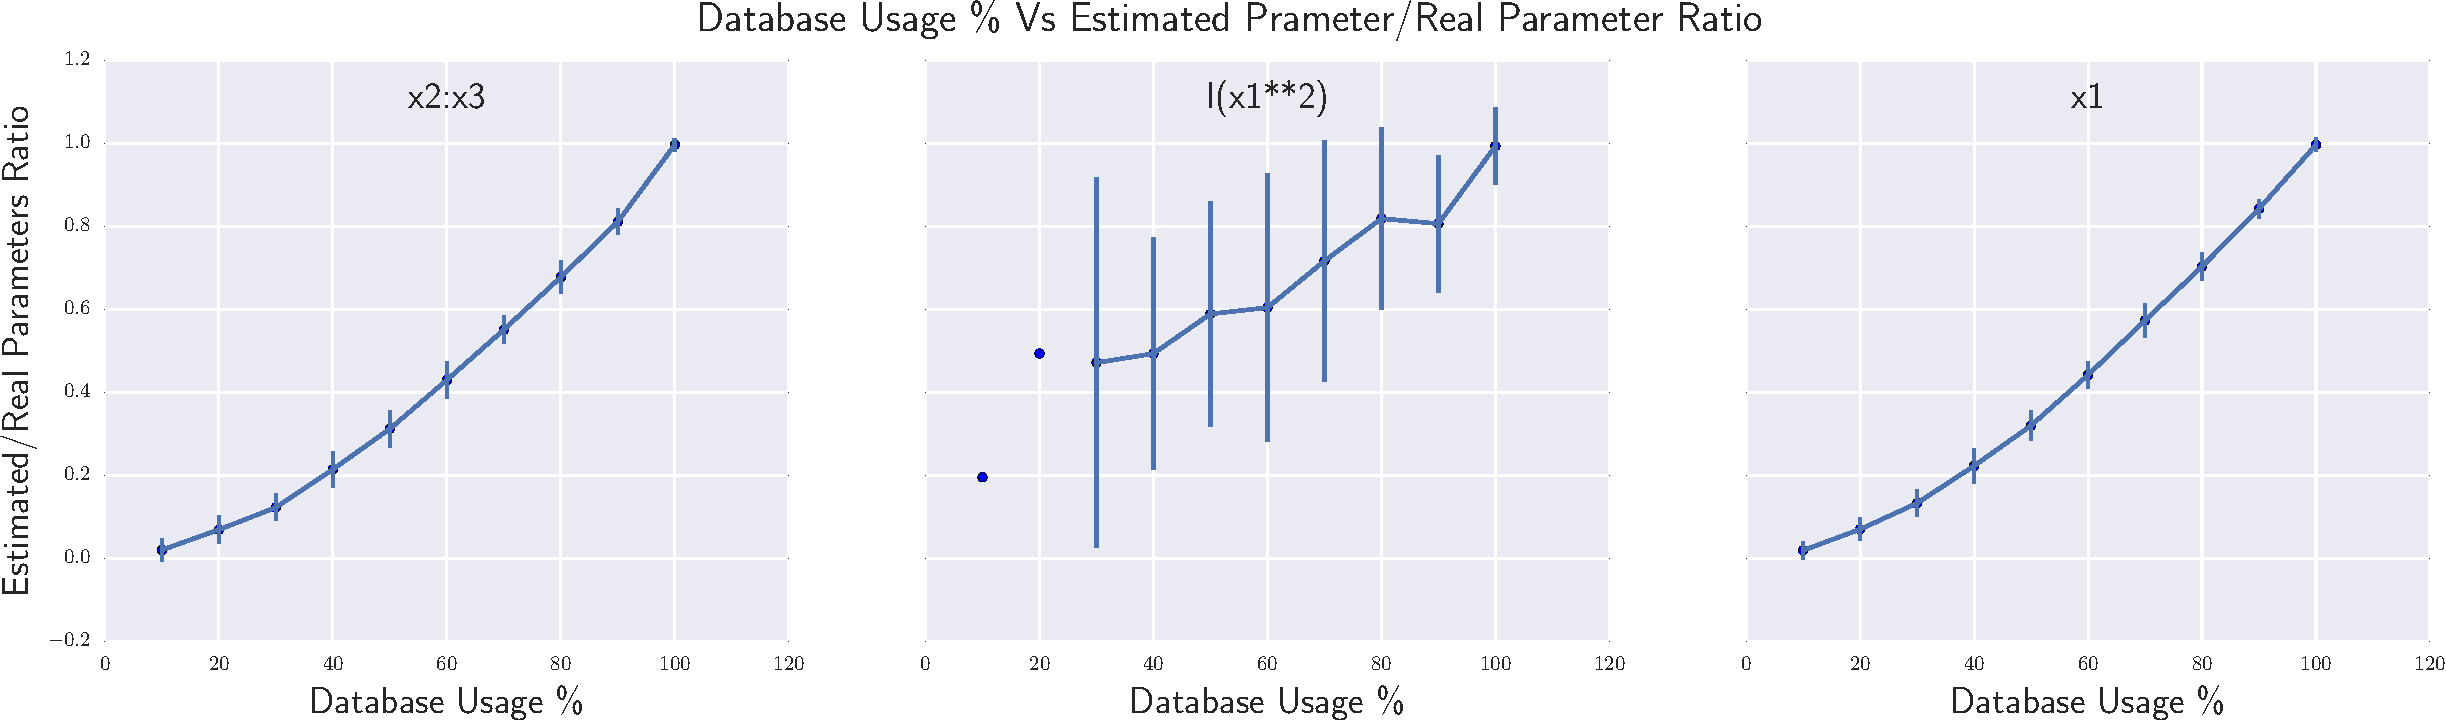
\includegraphics[width=1.0\linewidth]{finalgraph}
\caption{\textit{Plotting della variazione del rapporto fra coefficienti in relazione al taglio del dataset. Come è evidente dal grafico al centro l'errore aumenta considerevolmente per il parametro associato al termine di grado superiore al primo a causa della sua vicinanza allo zero.}}
\label{finalgraph}
\end{figure}

Si può notare come l'effetto della troncatura abbia nelle migliori delle ipotesi, ossia per un'analisi fatta con dati sintetici distribuiti normalmente, un'inferenza  estremamente consistente rappresentata dalla curva in figura \ref{finalgraph}.

\subsection{Conclusioni}
Alla luce della trattazione svolta in questo capitolo, è chiaro che i metodi comuni di analisi siano soggetti a forti deviazioni dovute ad una combinazione degli effetti descritti precedentemente.

Si hanno infatti oltre a fenomeni di \textit{leverage} facilmente ravvisabili (figura \ref{leverage}) e causa primaria dello spostamento delle rette di regressione, delle propagazioni anche in ambito di modelling e di stima dei coefficienti associati ai parametri.

Seppur in un'analisi del comportamento degli algoritmi canonici in relazione al ranking l'individuazione del corretto modello è generalmente mantenuta, la perdita di capacità predittiva relativa ai valori parametrici proporzionalmente alla perdita dei dati evidenzia la necessità dell'utilizzo di metodi di elaborazione dotati di una maggiore giustificazione analitica.

Nella prossima sezione saranno valutati gli effetti quantificati in questo capitolo in relazione all'applicazione a dati biologici reali.

In questo modo sarà possibile proporre una soluzione al problema dell'utilizzo dei metodi di classici tramite confronto, introducendo dei metodi che forniscano performance predittive migliori cercando di mantenere una certa semplicità operativa.

\chapter{Un ambito applicativo: Il Progetto Mark-Age}
\section{Uno sguardo al Progetto}
\subsection{Obiettivi}
Il progetto nasce in risposta al fatto che molti dei cosiddetti \textit{biomarcatori} per l'invecchiamento umano proposti dalla letteratura scientifica presentano una variabilità elevata per quanto riguarda gli studi trasversali.

Ciò implica che non sia ancora stato individuata una singola variabile che sussista da sola come marcatore utile per la determinazione dell'età biologica. Una spiegazione plausibile è data dall'intrinseca  natura \textit{multi-casuale} e \textit{multi-sistemica} dell'invecchiamento.



Lo scopo principale del progetto è quello di condurre uno studio di popolazione su circa 3200 soggetti per identificare in set di \textit{biomarcatori} per l'invecchiamento, i quali sotto forma di combinazioni di parametri a cui è attribuito un peso appropriato, siano complessivamente in grado di stimare l'età biologica in maniera più efficiente rispetto ad ogni tipo di marcatore isolato.

\subsection{Fondamenti teorici e strategie}
L'invecchiamento è stato definito come il declino dipendente dal tempo delle capacità funzionali e della resistenza agli stress, associato con il crescere del rischio di mortalità.
Il processo coinvolge la maggior parte dei tessuti e degli organi del corpo.

Inoltre è da considerare la trasversalità dei processi che avvengono tra molteplici sistemi fisiologici: ad esempio l'invecchiamento del sistema metabolico potrebbe influire sull'invecchiamento del sistema immunitario.

I meccanismi sottesi al processo, seppur originari del livello molecolare non escludono tassi di invecchiamento diversi all'interno della stessa specie animale, come ampiamente dimostrato; fenomeno da cui anche la specie umana non è esente. In altri termini, vi è differenza tra \textit{età biologica} ed \textit{età cronologica}.

La stima classica del tasso di invecchiamento è basata sull'analisi della \textit{curva di mortalità} (nota anche come funzione di Gompetz) per le popolazioni.

Questo però comporta che gli individui debbano essere monitorati fino alla conclusione delle proprie vite per determinare lo stato di invecchiamento biologico per ogni punto temporale della curva.

Riferendosi dunque ad un individuo vivente una valutazione plausibile dello stato di invecchiamento, come ad esempio lo stato definito dalla curva precedentemente citata, una predizione del rischio dell'aumento di probabilità di mortalità e una stima dell'aspettativa di vita residua non sono possibili all'interno di questo metodo.

Una strategia per la soluzione di questo problema è fornita dall'identificazione di cambiamenti legati all'età delle funzionalità corporee, che possano così fungere da misura dell'\textit{età biologica} e predire l'andamento ad esempio di malattie legate all'invecchiamento o stimare l'aspettativa di vita in maniera più precisa di quanto fornito dall'\textit{età cronologica}.

Questi cambiamenti sono i parametri definiti \textit{biomarcatori dell'invecchiamento}, chiamati così in analogia ai biomarcatori individuati per specifiche malattie croniche o relativi all'esposizione ad alcuni tipi di tossine.

I criteri per l'individuazione di un biomarcatore per l'invecchiamento sono posti dall'\textit{American Federation for Ageing Research}:
\begin{itemize}
\item Devono prevedere il tasso di invecchiamento più precisamente dell'età cronologica
\item Devono essere indicativi di processi sottesi all'invecchiamento, non di malattie
\item Dev'essere possibile effettuare test ripetuti senza danneggiare gli individui
\item I risultati devono essere compatibili per esseri umani e cavie da laboratorio
\end{itemize}

Il progetto su larga scala Mark-Age propone quindi uno studio su vasta popolazione per l'identificazione di biomarcatori efficaci dell'invecchiamento biologico all'interno di un range di diversi sistemi fisiologici.

La popolazione in analisi comprende 3200 soggetti comprensivi di diversi regioni geografiche europee, in uno span di età variabile tra i 35 e i 75 anni.

Sono stati presi in considerazione diversi possibili candidati biomarcatori, in quanto è ragionevole ipotizzare che una combinazione di diversi parametri possa costituire uno strumento d'analisi per la determinazione dell'età biologica rispetto all'isolamento di singole variabili.
Il processo di indagine tiene inoltre conto dei pesi effettivi che i diversi marcatori possono avere, in modo da evitare problemi legati alla normalizzazione dei risultati.

Una parte importante del progetto consiste dunque dell'ottimizzazione dei pesi per i marcatori utilizzando analisi multivariate.

Il reclutamento delle popolazioni è avvenuto in due larghi gruppi, il primo composto da 2262 \textit{randomly recruited age-stratified individuals from the general population (RASIG)} provenienti da differenti regioni europee, in numero eguale fra uomini e donne ed a numeri simili per gruppi d'età.
Questo gruppo è stato designato per rappresentare il tasso di invecchiamento medio di popolazione standard.

Il secondo gruppo è invece comprensivo di soggetti discendenti da rami familiari longevi, definiti \textit{Geha Offspring (GO)} e con età nel range dei 55-74 anni.
Ciò per confermare le ipotesi presenti in letteratura riguardanti un più basso tasso di invecchiamento per questi individui geneticamente peculiari.

All'interno del progetto inoltre i soggetti GO vengono confrontati con i loro coniugi, definiti \textit{Spouses of Geha Offspring (SGO) } poiché il paragone sistematico dei due gruppi costituisce un'opportunità di prima validazione per i biomarcatori individuati trasversalmente per i soggetti RASIG.
Ci si aspetta infatti che i GO mostrino in generale un'età biologica inferiore rispetto ai loro coniugi.

Di tutti gli individui analizzati sono stati raccolti dati antropometrici, clinici e demografici in maniera standardizzata.
Una lista dettagliata di tutti i tipi di dati raccolti per ogni macro-categoria citata sopra è presente nell'articolo in letteratura \cite{markage}.

A causa della considerevole mole di dati clinici e biochimici  raccolti all'interno del progetto, è obbligatoria una rigorosa ed appropriata strategia di analisi e costruzione dei modelli.

Per far fronte a questa esigenza ed estrarre un set valido di biomarcatori dell'invecchiamento sono state eseguite le seguenti procedure:
\pagebreak
\begin{itemize}
\item \textbf{Analisi della consistenza dei dati}

E' stata utilizzata la conoscenza pregressa a proposito di correlazioni fra variabili ipotizzate per giudicare il rapporto del rumore per alcune delle misure usando metodi statistici classici.
Per una robustezza ancora maggiore alcuni campionamenti sono stati ripetuti nell'arco di sei mesi.
\item \textbf{Tecniche di Modelling}

Sono stati utilizzati metodi statistici, di machine learning e di data mining per la costruzione di modelli in grado di predire nel migliore dei modi possibili l'età biologica.
Sono state impiegate tecniche classiche come  l'analisi di regressione ma anche metodi di Networking Neurale per acquisire una migliore conoscenza delle proprietà \textit{locali} delle interazioni fra le variabili.

\item \textbf{Riduzione della Varianza}

L'obiettivo è quello di ridurre le misure necessarie ma allo stesso tempo ridurre la varianza delle predizioni generate attraverso tecniche di riduzione dimensionale (quali ad esempio analisi della principale componente).
Il machine learning gioca un ruolo fondamentale per questo aspetto.

\item \textbf{Clustering e visualizzazione}

Ci si aspetta di individuare nuove relazioni fra i dati nell'individuazione della corretta età biologica.
I metodi di visualizzazione interattiva e di clustering costituiscono uno strumento agevole per la scoperta di nuove correlazioni.
E' infatti ipotizzato che alcuni tipi di misure abbiano una maggior correlazione con l'età biologica rispetto ad altri.
L'individuazione di cluster di questo tipo di parametri aiuta a ridurre la varianza dei modelli generati, in quanto si avranno caratteristiche migliori per i modelli generati da sub sets di dati.

\end{itemize}
\pagebreak

\subsection{Un possibile caso analitico}
Di seguito è riportato un esempio di analisi di regressione utilizzando alcuni dei dati clinici raccolti all'interno del progetto, esplicativo delle più comuni tecniche di elaborazione elencate sopra.

Nello specifico è data la rappresentazione dei risultati delle previsioni a seguito di un'interpolazione con regressione multivariata di due variabili e delle relative interazioni.
Per raffinare l'indagine è stato introdotto uno script esecutivo per il train-test split dei datasets all'interno di un ciclo, in modo da poter ottenere un'elaborazione statistica per correlatori, residui ed errori.

E' stata proposta in questo caso l'interpolazione lineare di due labels spirometriche, il \textbf{flusso di picco espiratorio (PEF)}, misurato in litri al secondo (l/s) ed il \textbf{volume espiratorio forzato (FEV)}, misurato in litri. 
E' stata utilizzata questa classe di parametri in quanto nota la sua teorica correlazione con l'età biologica. 
Nella regressione multivariata, oltre alle due variabili PEF e FEV sono state considerate le reciproche interazioni, secondo un modello del tipo $Y=AX_1+BX_2+C(X_1*X_2)+D$.
La popolazione osservata è quella dei soggetti di tipo \textit{RASIG} di entrambi i sessi.

\begin{figure}[!h]
\centering
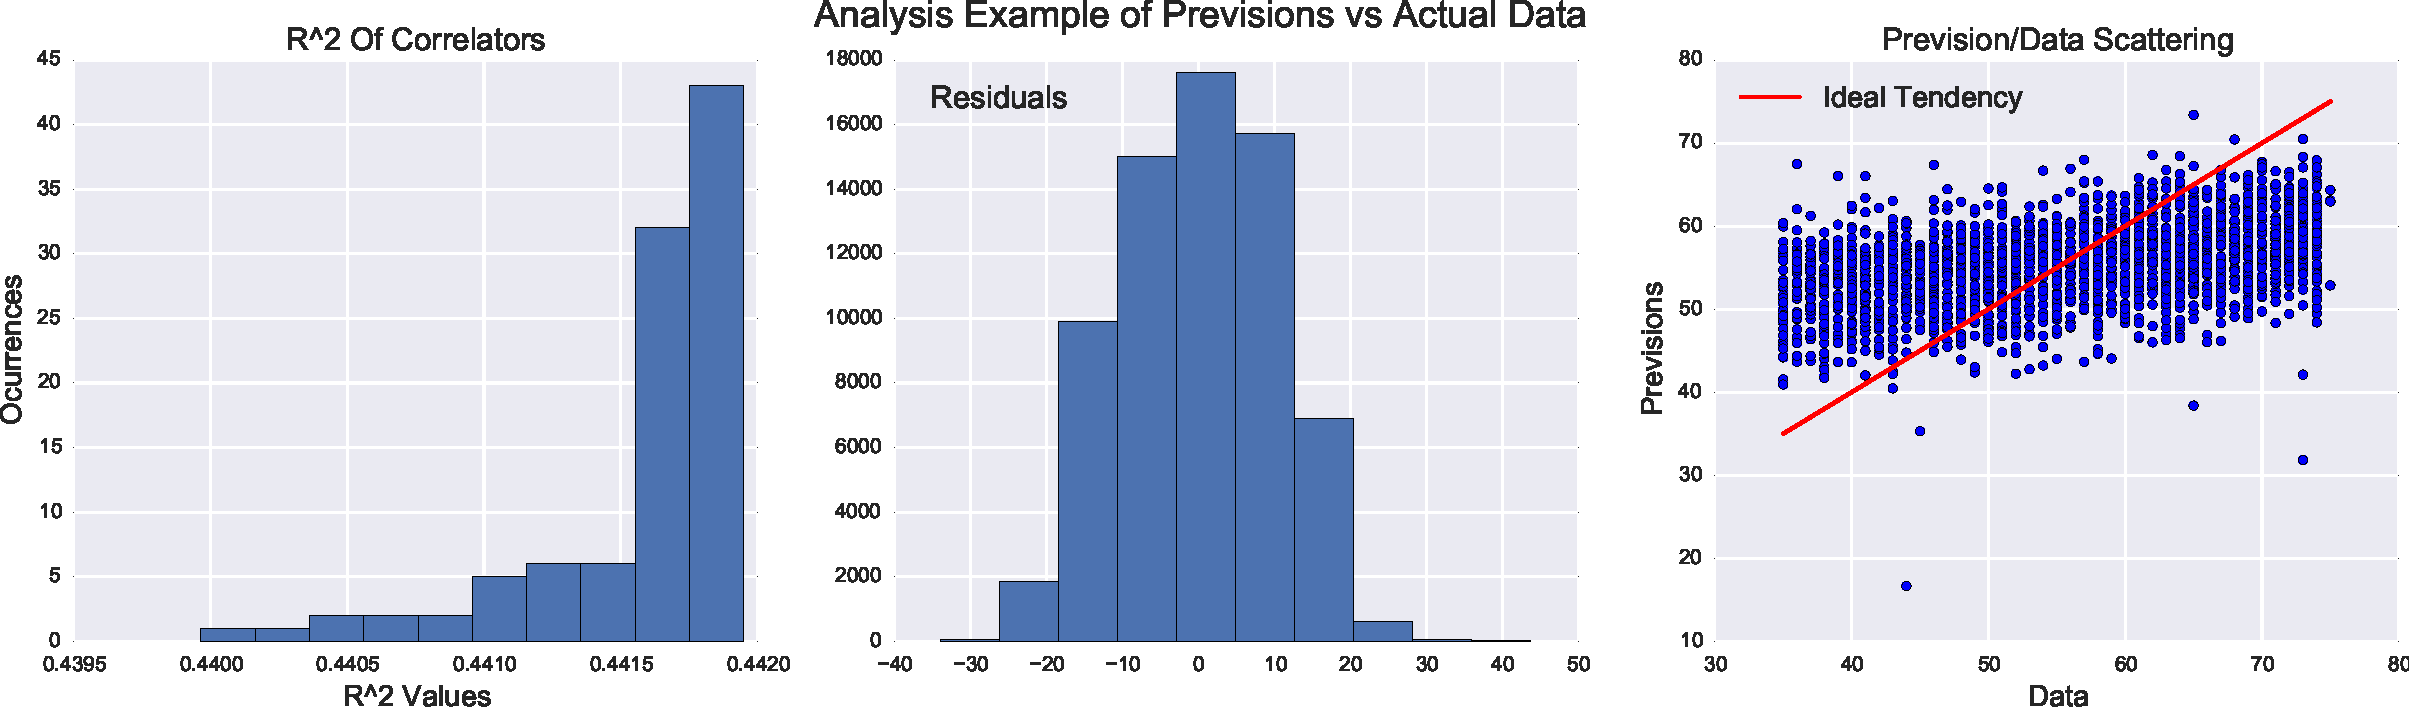
\includegraphics[width=1.2\linewidth]{mulregression}
\caption{\textit{Lo scatter plot finale rappresenta la coincidenza tra valori di età previsti, cioè calcolati dal modello, e valori di età noti degli individui. Qualora questa fosse perfetta, avremmo la tendenza indicata dalla retta in rosso.}}
\label{mulregression}
\end{figure}

Come immediatamente risalta dalla figura \ref{mulregression}, oltre ad un basso valore di $R^2$ per i correlatori, elaborato come media statistica delle occorrenze e con un valore pari a $0.4415\pm0.0004$ indicativo di una scarsa performance predittiva per questo caso analitico, la distribuzione dei residui è molto piccata.

Quest'ultimo fatto è sintomatico dell'effetto di troncatura deterministica dovuto al criterio di selezione dello span di età, quantificato nel grafico \ref{finalgraph} per il calcolo dei coefficienti.

Si ha in questo modo la perdita delle condizioni di normalità della distribuzione necessaria all'utilizzo del metodo dei mini quadrati nel calcolo del MLE.

Come è evidente poi dalla figura \ref{leverage}, l'effetto di spostamento della pendenza della retta di regressione è consistente per database troncati deterministicamente.
Questo fenomeno è immediatamente ravvisabile anche per l'analisi effettuata in figura \ref{mulregression}, ove emergono nettamente i margini di troncatura dati dal criterio di selezione dello span di età per gli individui campione.

Nella prossima sezione seguirà pertanto il necessario confronto operativo fra metodi classici di regressione e metodi analiticamente corretti.

\section{Risultati dell'elaborazione con metodo corretto}

L'elaborazione data dalla Figura \ref{mulregression} evidenzia la presenza degli effetti trattati nel Capitolo 2 anche per dati sperimentali.
Ciò costituisce una prova a favore della scarsa consistenza delle ipotesi analitiche per i minimi quadrati ordinari nel caso in cui i dati siano troncati.

Va introdotto dunque un metodo in grado di utilizzare una funzione di massima verosimiglianza che tenga conto della troncatura.

Viene utilizzato quindi per l'elaborazione un algoritmo basato sul cosiddetto modello \textit{Tobit}, il quale introduce l'ipotesi di una variabile latente (cioè non osservabile) $\tilde{y_i}$.
Questa è dipendente dalla $x_i$ tramite un parametro (o vettore) $\beta$, indicativo della correlazione fra le due variabili.

Si suppone inoltre la presenza di un rumore statistico $u_i$ distribuito normalmente; si definisce inoltre la variabile $y_i$, cioè la osservabile, coincidente con la $\tilde{y_i}$ ogniqualvolta la variabile latente sia al di sopra dello zero.

\begin{equation}
y_i = \begin{cases} 
    \tilde{y_i} & \textrm{if} \; \tilde{y_i} >0 \\ 
    0     & \textrm{if} \; \tilde{y_i} \leq 0
\end{cases}
\end{equation}

Con $\tilde{y_i}$ data da 

\begin{equation}
\tilde{y_i} = \beta x_i + u_i, u_i \sim N(0,\sigma^2) \, 
\end{equation}

Se il parametro $\beta$ fosse stimato tramite una la regressione delle $y_i$ per le $x_i$, l'estimatore dato dai minimi quadrati ordinari risulterebbe inconsistente. 

$\beta$ non va infatti interpretato come l'effetto delle $x_i$ sulle osservabili $y_i$, come nel caso dell'interpretazione lineare classica.
Esso rappresenta la combinazione della variazione del valore delle $y_i$ sopra il limite, pesata tramite la \textit{probabilità di essere al di sopra del limite}, e la variazione nella probabilità di essere al di sopra del limite, pesata tramite il \textit{valore di aspettazione} delle $y_i$ al di sopra del limite. \cite{tobit}

Vi sono varie classificazioni di modelli tobit, relative alla variazione degli intervalli di taglio; per gli scopi di questo lavoro è stato utilizzato un modello tobit detto di \textit{tipo 1}, definito come

\begin{equation}
 y_i = \begin{cases} 
   \tilde{y_i} & \textrm{if} \; y_L<\tilde{y_i}<y_U \\ 
    y_L   & \textrm{if} \; \tilde{y_i} \leq y_L \\
    y_U   & \textrm{if} \; \tilde{y_i} \geq y_U
\end{cases}
\end{equation}

dove cioè i limiti del taglio $y_L$ e $y_U$ sono valori discreti diversi da zero.

Una sistematica delle soluzioni consistenti per la maximum likelihood di questo e di altri tipi di modelli tobit è presente in letteratura \cite{tobitMLE}.

Per l'elaborazione dei risultati seguenti è quindi stato utilizzato uno script basato su questa particolare variazione del modello, in quanto i campioni del progetto Mark-Age sono stati raccolti all'interno di un range di età definito (35-75 anni), equiparabile dunque ai limiti $y_L$ ed $y_U$.

E' stata scelta come variabile di prova la cosiddetta \textbf{FVC} o \textit{forced vital capacity}, misurata in litri, in quanto nota la sua relativa correlazione con l'età biologica per un soggetto sano.
La popolazione di campionamento per questa analisi è quella dei \textit{RASIG} di ambo i sessi, essendo comprensiva della maggior parte delle osservazioni all'interno del database del progetto.

Il risultato dell'introduzione del modello tobit è riportato in figura \ref{truncatedml}.
Notiamo immediatamente come la retta di regressione calcolata con il metodo dei minimi quadrati ordinario sia soggetta ad un forte fenomeno di \textit{leverage}, causato dal troncamento di cui il metodo OLS non tiene conto.

La retta di regressione calcolata tramite la maximum likelihood per il modello tobit, a cui è associato un intervallo di confidenza standard proprio dell'algoritmo, ha una pendenza e dunque un andamento estremamente più plausibile al di fuori dei limiti di taglio (peraltro molto evidenti nello scatter plot). 
L'effetto di \textit{leverage} è in questo modo compensato.

Si nota inoltre come il metodo OLS preveda dei valori discreti per i parametri di regressione ed il calcolo della deviazione standard, nonostante questi siano comunque elaborati statisticamente (vi sono infatti nello script cicli che permettono di ripetere le analisi ed utilizzare le medie come valori veri).

Il metodo tobit invece, a causa della definizione dei parametri $\beta$ riportata nella trattazione precedente, fornisce per slope, intercetta e deviazione standard degli intervalli probabilistici.
Confrontando i range con i valori discreti forniti dal metodo OLS appare visibilmente come questi ultimi si distanzino fortemente dalle distribuzioni date dal modello tobit.

E' perciò evidente ancora una volta la presenza di effetti di \textit{leverage} combinata con la perdita di precisione nella stima dei parametri quantificata dalla figura \ref{finalgraph} per il caso dei minimi quadrati ordinari.


\begin{figure}[!h]
\centering
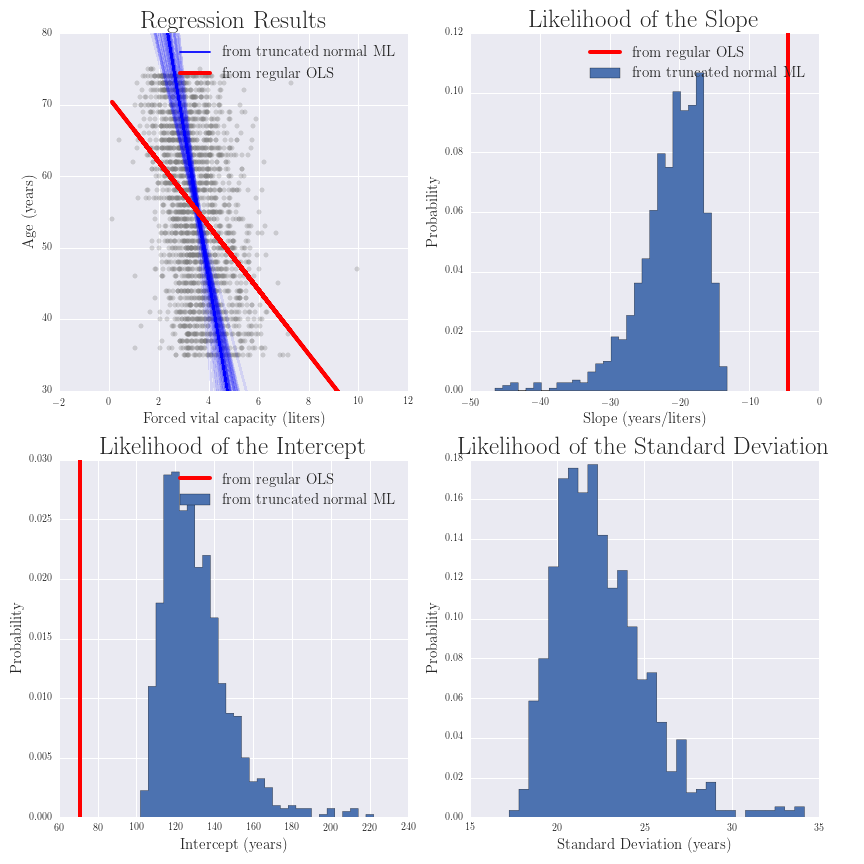
\includegraphics[width=1.0\linewidth]{truncatedml}
\caption{\textit{I grafici in figura sono rappresentativi del confronto con il metodo classico (OLS).
L'introduzione di un metodo analiticamente consistente come il tobit evidenzia lo spostamento della retta di regressione dovuto al troncamento, oltre al fatto che i parametri di regressione (Slope,Intercept) e deviazione standard assumono ora la forma di un range probabilistico.}}
\label{truncatedml}
\end{figure}

D'altra parte, l'introduzione di un metodo analiticamente giustificato come il tobit permette invece di sopperire alle inferenze sulla performance predittiva del modello lineare descritte e quantificate nel Capitolo 2.

\backmatter
\begin{thebibliography}{99}
\bibitem{ESL}
Trevor Hastie, Robert Tibshirani, Jerome Friedman

\emph{The Elements of Statistical Learning}
Springer ISBN 978-0-387-84858-7

\bibitem{fornasini}
Fornasini, Paolo

\emph{The Uncertainity in Physical Measurement}
Springer ISBN 978-0-387-78650-6

\bibitem{Mdata}
Enders, Craig K. (2010)

\emph{Applied Missing Data Analysis } (1st ed.)
 New York
 Guildford Press ISBN 978-1-60623-639-0.

\bibitem{MLE}
Hazewinkiel, Michel

\emph{"Maximum Likelihood Method", Encyclopedia of Mathematics}
Springer ISBN 155608000X

\bibitem{TGMLE}
Johnson, Kotz, Blakrishnan

\emph{Continuos Univariate Distributions, Volume 1}
Wiley ISBN 0471584959 

\bibitem{econ}
Amemiya, Takeshi 

\emph{Regression Analysis when the Dependent Variable is Truncated Normal}
Econometrica, Novembre 1976,Volume 41, Numero 6  DOI 10.2307/1914031

\bibitem{markage}
Burkle, A. et al.

\emph{MARK-AGE biomarkers of ageing} 
Mech. Ageing Dev. (2015) http://dx.doi.org/10.1016/j.mad.2015.03.006

\bibitem{tobit}
Amemiya, Takeshi 

\emph{Tobit models: A survey}
 Journal of Econometrics 24 (1–2): 3–61. doi:10.1016/0304-4076(84)90074-5

\bibitem{tobitMLE}
Schnedler, Wendelin

\emph{Likelihood estimation for censored random vectors}
Econometric Reviews 24 (2): 195–217. doi:10.1081/ETC-200067925

\end{thebibliography}


\end{document}